

%exp_9.tex
\documentclass[]{article}
\usepackage{multirow}
\usepackage{graphicx}
\usepackage{amsmath}
\begin{document}
\section{Number of the reference}
The results are shown in Table \ref{fig:de}.
\begin{table}[htbp]
	\caption{department.}\label{fig:de}\begin{tabular}{c|c} 
		\hline School of& Information and Communication Engineering	\\
		\hline c& d	\\ 		\hline 
\end{tabular}\end{table}	 
\par{}The results are shown in Figure \ref{fig:bup}.
\begin{figure}[ht]
	\caption{Beijing University of Posts and Telecommunications}\label{fig:bup}
	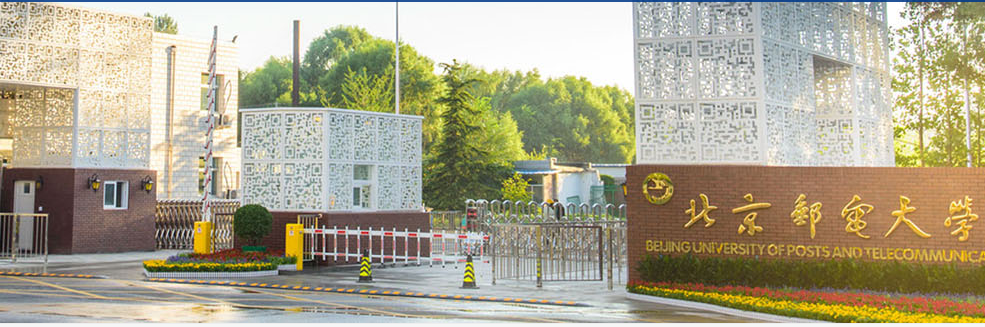
\includegraphics[width=13cm]{bupt.png}
\end{figure}
\par{}From Formula (\ref{eq:con}), we can get that \dots
\begin{equation}\label{eq:con}
{{\text{X}}_s} \subseteq {\rm E}{\text{X}}{\rm P}{{\text{R}}_{\text{s}}}{\text{  }}for{\text{ }}every{\text{ }}s \in {\text{S}}
\end{equation}
\end{document}